

\subsection{Statistical uncertainty}
\label{subsec:statuncertainty}
To account for statistical uncertainty, the data normalisation was
thrown according to a Poisson distribution of parameter the number
events expected. Similarly, for the \Gls{MC} statistic uncertainty,
same procedure was applied without any weight nor correction or
tuning. Doing this, one finds that the relative statistical
uncertainty is \datastaterror for the data, and \mcstaterror for the
\Gls{MC}. The effect on the selected events is shown in
Figure~\ref{fig:statuncertainty}.

\begin{figure}[ht]
  \begin{adjustbox}{center}
    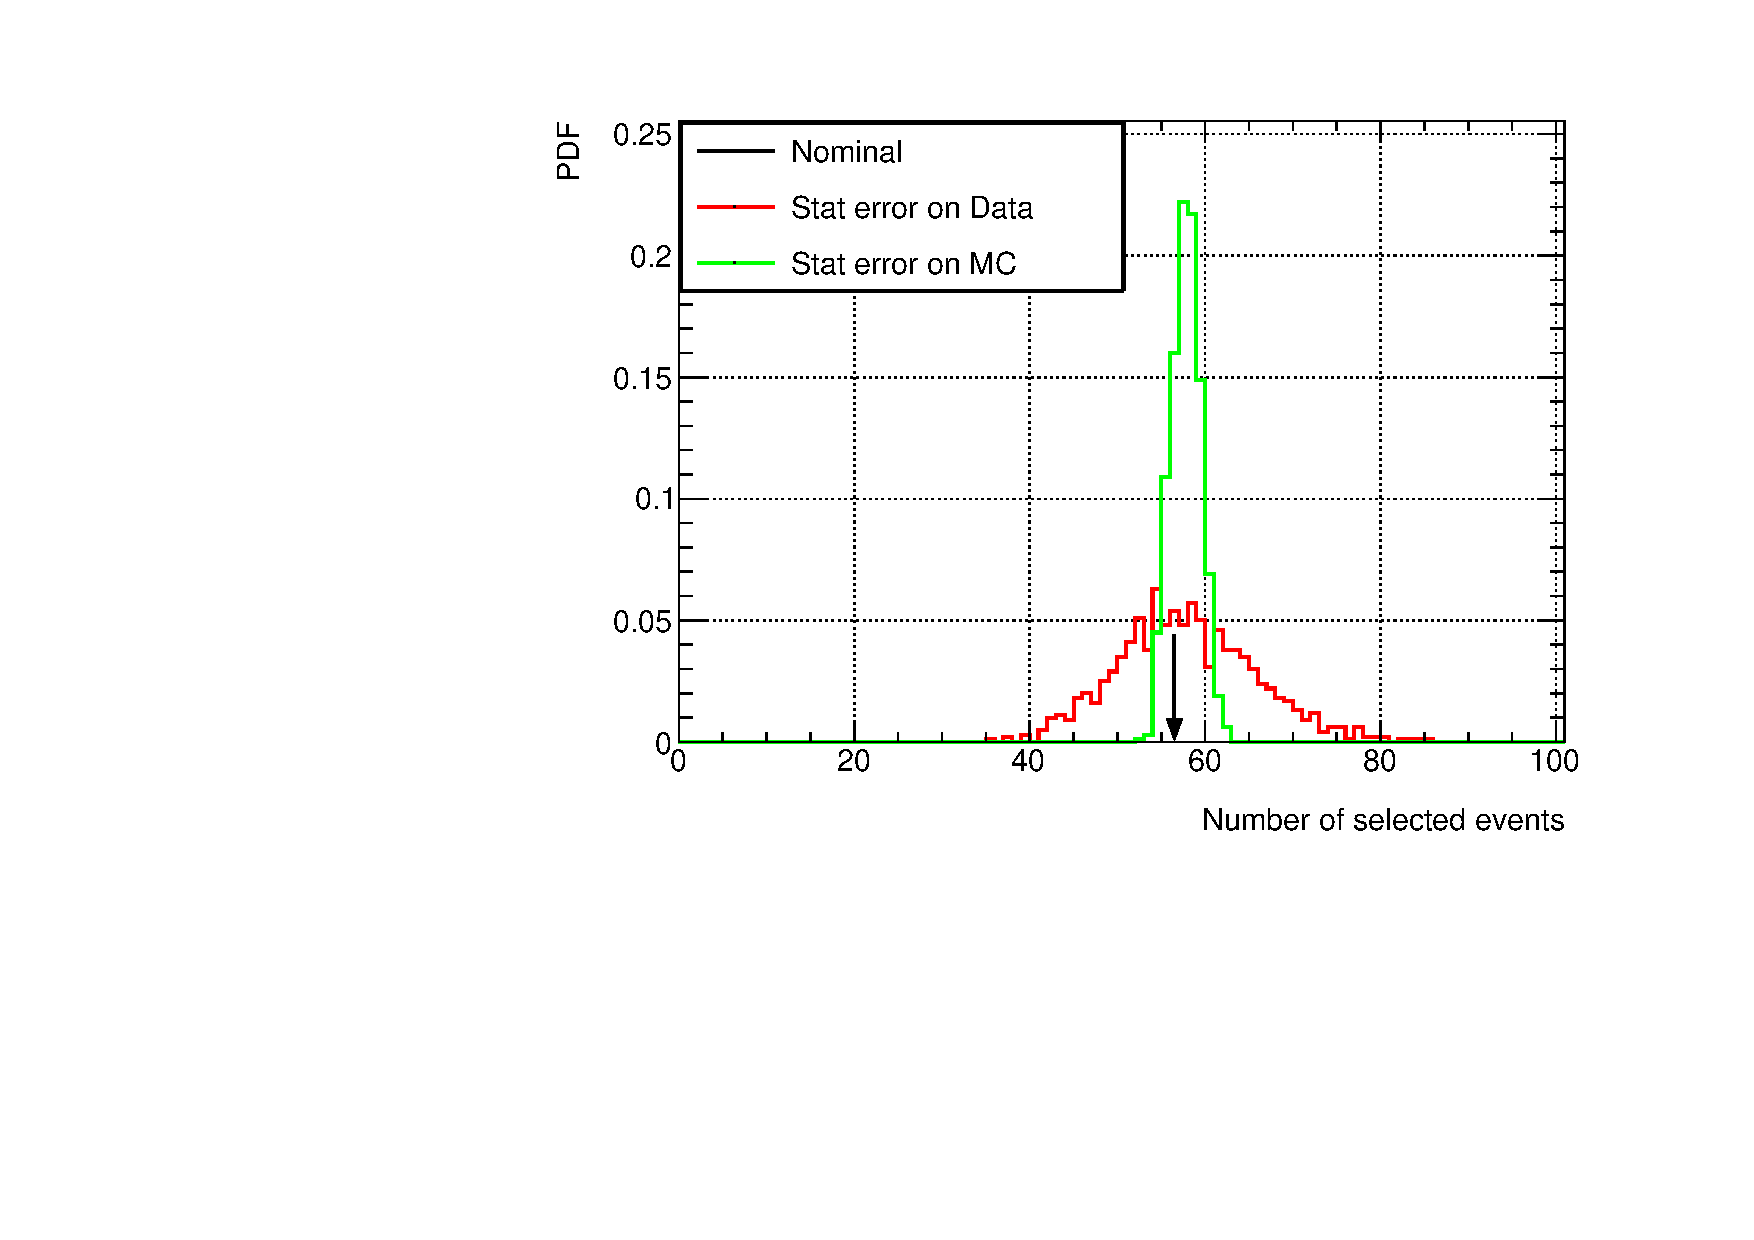
\includegraphics[width=0.8\textwidth]{images/NCg/stat.pdf}
  \end{adjustbox}
  \caption[Effect of all the statistical uncertainties on the number
  of selected events]{Effect of all the statistical uncertainties
    (data and \Gls{MC}) on the number of selected events. The nominal
    central value is indicated by the arrow.}
  \label{fig:statuncertainty}
\end{figure}

\subsection{Efficiency uncertainty}
\label{subsec:effuncertainty}
The efficiency also has an systematic error associated to it. To get
it, the statistical uncertainty on the number of events selected after
all the cuts is computed (simply the square root of the number of
event divided by the number of event selected).  To do this, a very
high \Gls{POT} of \Gls{NCg} events have been generated
($6.5\times 10^{24}$ \Gls{POT}).

\subsection{Combination of asymmetric error}
\label{subsec:combinationerror}
To combine all the systematic errors and get a toy distribution
allowing a proper treatment of the very asymmetric detector error that
was discussed in the previous sections, a ``discrete convolution
method'' was proposed, this method is now described.

All the independent errors were thrown, including the Poisson
statistical uncertainty of the data and MC. In a standard cross
section analysis where all the errors that are Gaussian, the errors
are then added in quadrature and get the number of event at 90\%
\Gls{CL}, $N_\text{events}^{90\%CL}$, by integrating:
\begin{equation}
\label{eq:integral}
0.90 = \int^{N_\text{events}^{90\%\text{CL}}}_{-\infty}\text{Gauss}\left(\mu = N_\text{events}^\text{nominal}, \sigma \right) dN_\text{events},
\end{equation}
where $N_\text{events}^\text{nominal}$ is the nominal number of events
after all the correction and tuning, and $\sigma$ is the total
uncertainty on this number after summing all the independent errors in
quadrature.

Note that the assumption that one can add the errors in quadrature is
central in this method. However, it cannot be applied for asymmetric
errors as is the case in this analysis.

Rather than adding the errors in quadrature, the ratios
$N_\text{events}^\text{toy} / N_\text{event}^\text{nominal}$ were
computed for each toy and for each uncertainty source. To get the
total \Gls{PDF} (Probability Distribution Function) of the number of
selected events, one just has to multiply all these ratios with each
other:
\begin{equation}
\label{eq:toycombination}
N_\text{events}^\text{toy} = N_\text{event}^\text{nominal} \times \prod_{i = \text{source}}\prod_{j = \text{toy}}
\frac{N_\text{events}^{\text{toy} i,j}}{N_\text{events}^\text{nominal}},
\end{equation}
where $i$ denotes the source of the uncertainty (it can be detector,
flux, \Gls{FSI}, cross section, data or \Gls{MC} statistics), and $j$
is the particular toy. In practice, the number of toy experiments
grows exponentially with the number of source of systematic errors,
therefore the systematic uncertainties with Gaussian behaviour (flux,
cross section, \Gls{FSI}, data and \Gls{MC} statistics) were added in
quadrature and used to generate 1000 toy experiments to combine with
the asymmetric detector uncertainty as described earlier.

\subsection{Effect of all uncertainties}
When combining the uncertainties as described in the previous section,
one obtains the distribution shown in Figure~\ref{fig:allsyst}.

\begin{figure}[ht]
  \begin{adjustbox}{center}
    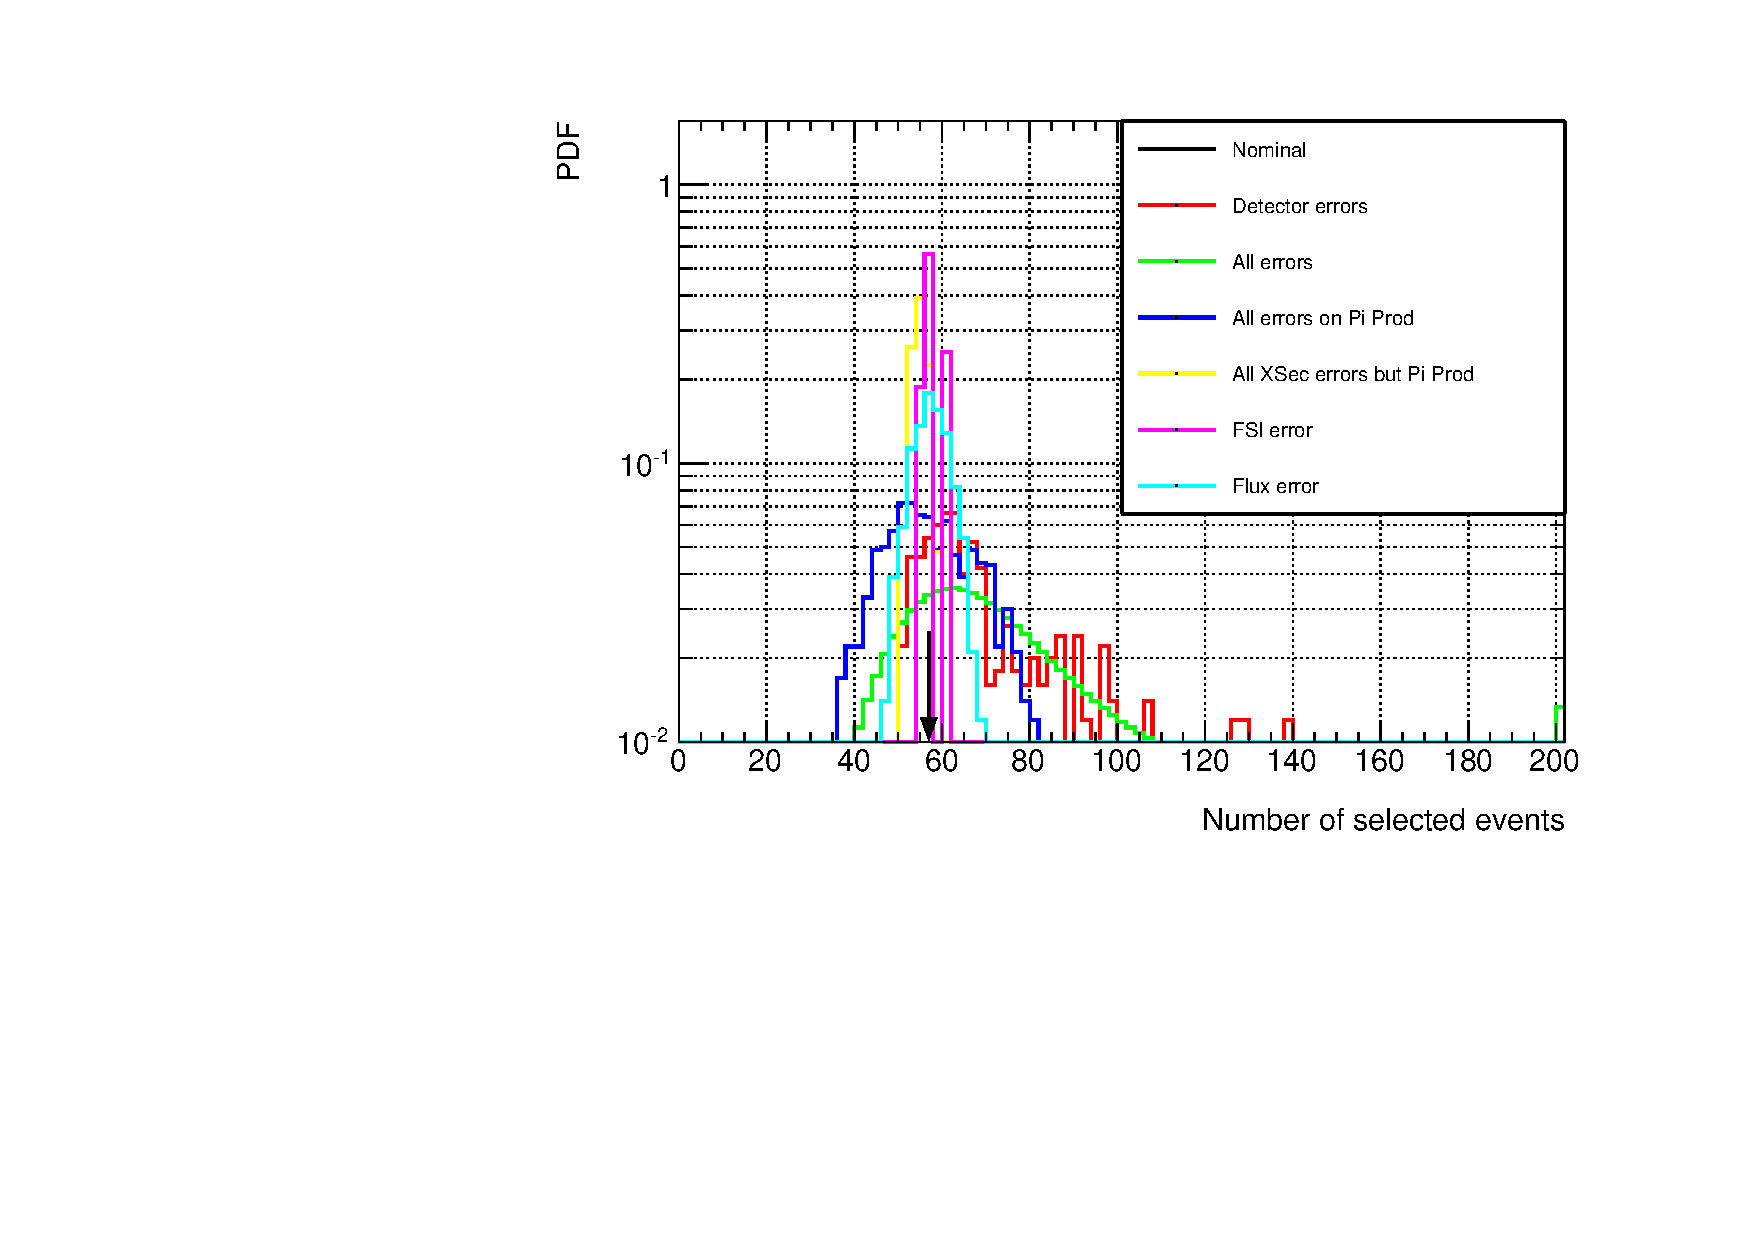
\includegraphics[width=0.8\textwidth]{images/NCg/All.pdf}
  \end{adjustbox}
  \caption{Effect of all the uncertainties in the total number of
    selected events.}
  \label{fig:allsyst}
\end{figure}

Note, that as can be seen in Figure~\ref{fig:detectorsystematicsinfv},
the detector systematic uncertainties introduce a relatively large
bias towards higher number of events. This bias gets propagated on the
total systematic uncertainty distribution (``All errors'' on
Figure~\ref{fig:allsyst}), but not on the other distributions (cross
section errors, \Gls{FSI}, flux). This is why the error on pion
production \Gls{PDF} seems to extend towards lower number of events
than the one with all the errors. It was checked that appling the same
bias to the pion production error gives shifts the pion production
error \Gls{PDF} under the one with all the errors.

\subsection{\texorpdfstring{Motivation of the $\varphi_\text{photon}$ cut}%
  {Motivation of the photon phi cut}}
\label{subsec:downwardphotons}

An interesting feature is exhibited in Appendix~\ref{app:mass}, for
bottom-originated events, there is a higher uncertainty than for the
rest of the selection (Table~\ref{tab:oofvmasserror}). Since the
pointing capabilities of the \Gls{FGD}1 is reasonably good for event
coming from all the directions (see Appendix~\ref{app:rec}), one can
restrict the phase space to events originated from the top and the
side directions. This is done with a simple cut on the $\varphi$ angle
of the reconstructed photon direction.  The effect of adding this
phase space cut is shown in Figure~\ref{fig:detectorphi}.

However, such a cut would have an impact too drastic on the efficiency
and on the statistics of the selected events. So, rather than removing
all the events from the downward direction, the cut was optimised. To
do that, the only uncertainties of interest are the detector
systematic errors and the data statistical error. Similarly, the
efficiency is going to decrease if one removes too many events from
downward. The optimisation of this cut was performed by minimising its
value by minimizing the value $N_\text{Signal}/\epsilon$

In this ratio, $N_\text{Signal}$ is the difference between the 90\%
upper \Gls{CL} of the number of \Gls{MC} events and the nominal number
of events (which essentially gives an idea of the uncertainty) and
$\epsilon$ is the efficiency. The Figure~\ref{fig:optimisationphi}
motivates the chosen value of $\varphi_\text{cut} = 36^{\circ}$. This
value is then translated for the excluded angles
$\varphi_{\text{photon}}$:

\begin{align}
  -90^{\circ} - \varphi_{\text{cut}} / 2 &< \varphi_{\text{photon}} < -90^{\circ} + \varphi_{\text{cut}} / 2 \\
  -108^{\circ} & <  \varphi_{\text{photon}} < -72^{\circ}.
\end{align}

All the errors are depicted in Figure~\ref{fig:allsystphi} and
summarised in Table~\ref{tab:AllErrorPhiCut} after this cut (called
$\varphi_\text{photon}$ cut from now on). Note that in this table, the
positive and negative errors are determined using the \Gls{HPD}
(Highest Posterior Density) method (see Footnote~\ref{ftn:hpd} on
page~\pageref{ftn:hpd}). As explained earlier, this method is quite
sensitive to the number of toy thrown and the binning chosen for the
computation. For example, it fails in giving a reasonable answer for
the \Gls{COH} cross section error, since the highest probability is at
the edge of its \Gls{PDF}. Therefore, only the detector and the total
errors have been computed using this method.

\begin{figure}[ht]
  \begin{adjustbox}{center}
    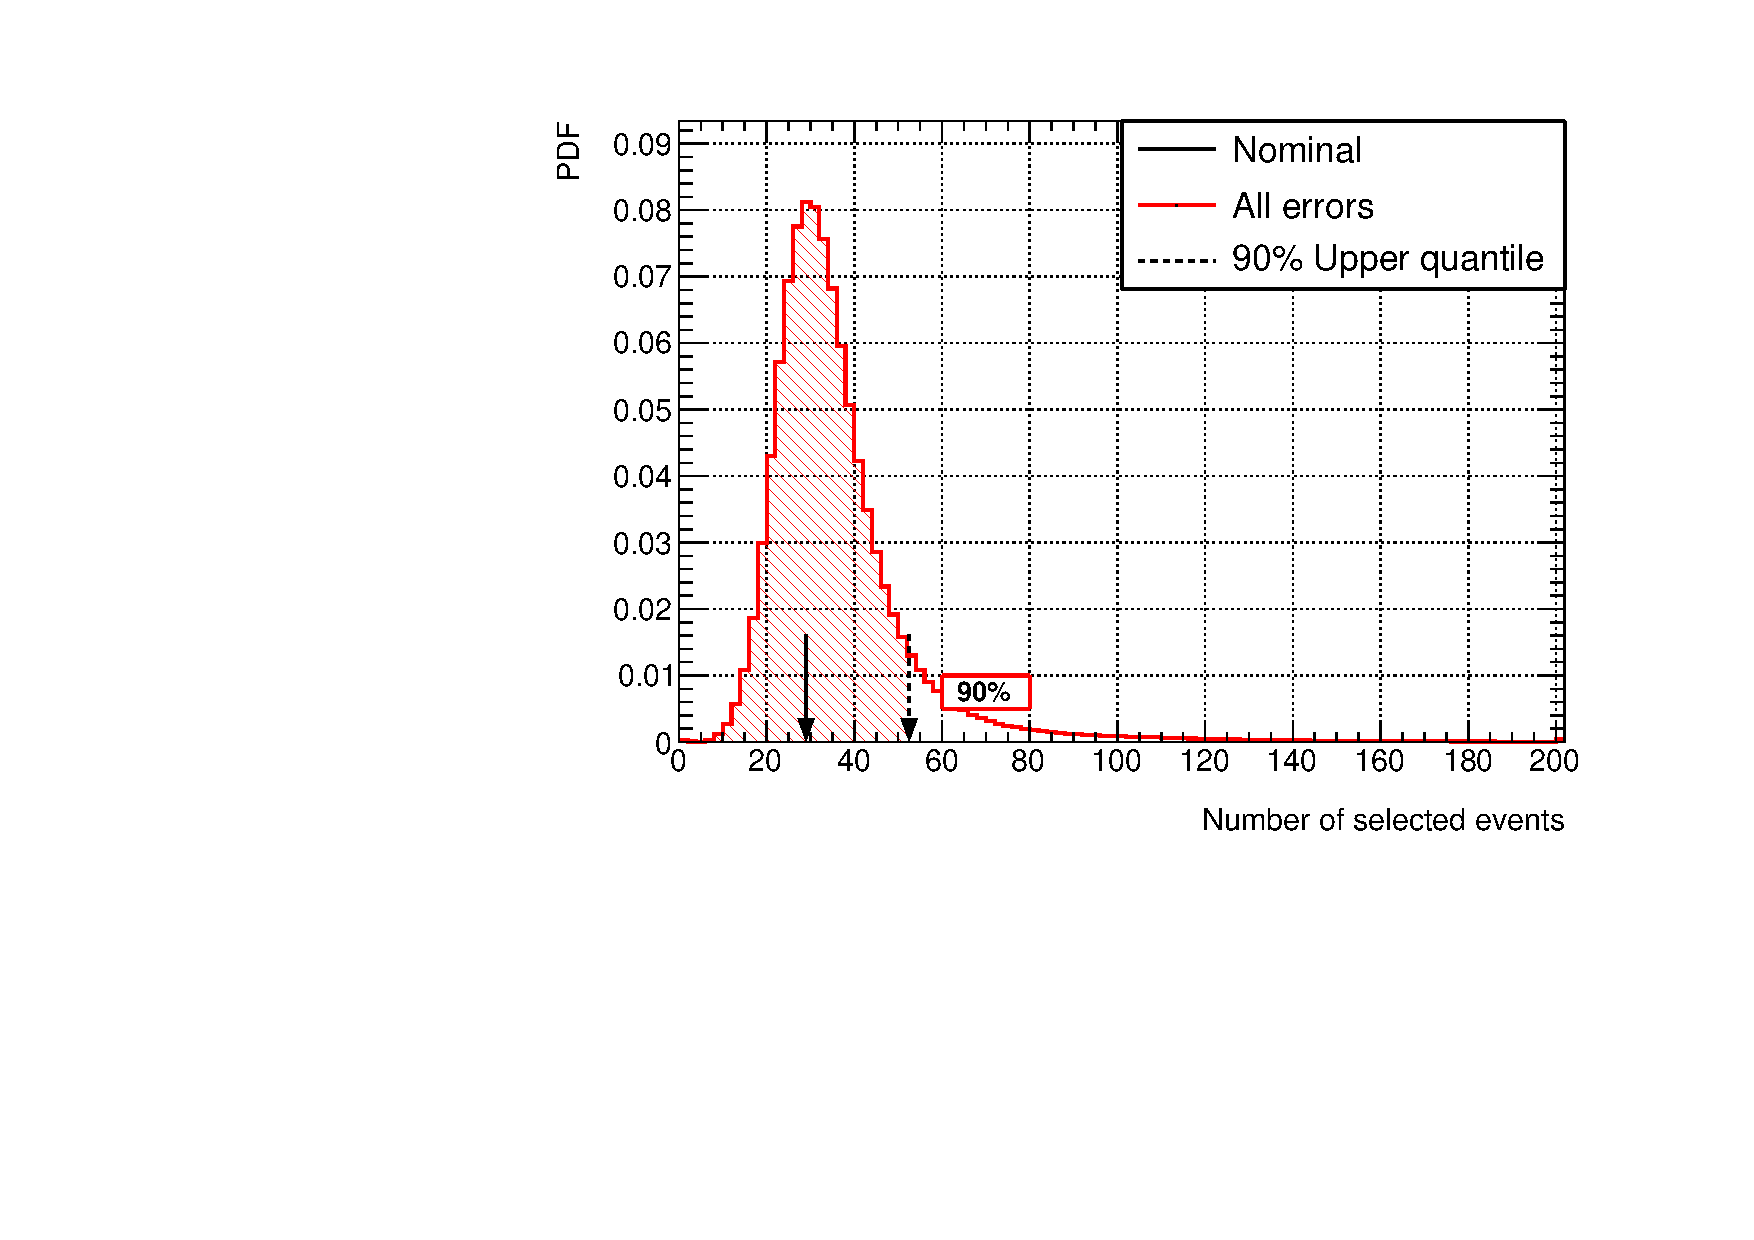
\includegraphics[width=0.8\textwidth]{T2K-TN-254/images/systematics/QuantilePhiBTZ.pdf} 
  \end{adjustbox}
  \caption[PDF of the selected number of events from the detector
  uncertainties after the azimuthal cut ($\varphi > 0$)]{\Gls{PDF} of
    the selected number of events from detector uncertainties
    (including the \Gls{OOFV} one) after the azimuthal cut
    ($\varphi > 0$). The nominal central value is indicated by the
    arrow.}
  \label{fig:detectorphi}
\end{figure}

\begin{figure}[ht]
  \begin{adjustbox}{center}
    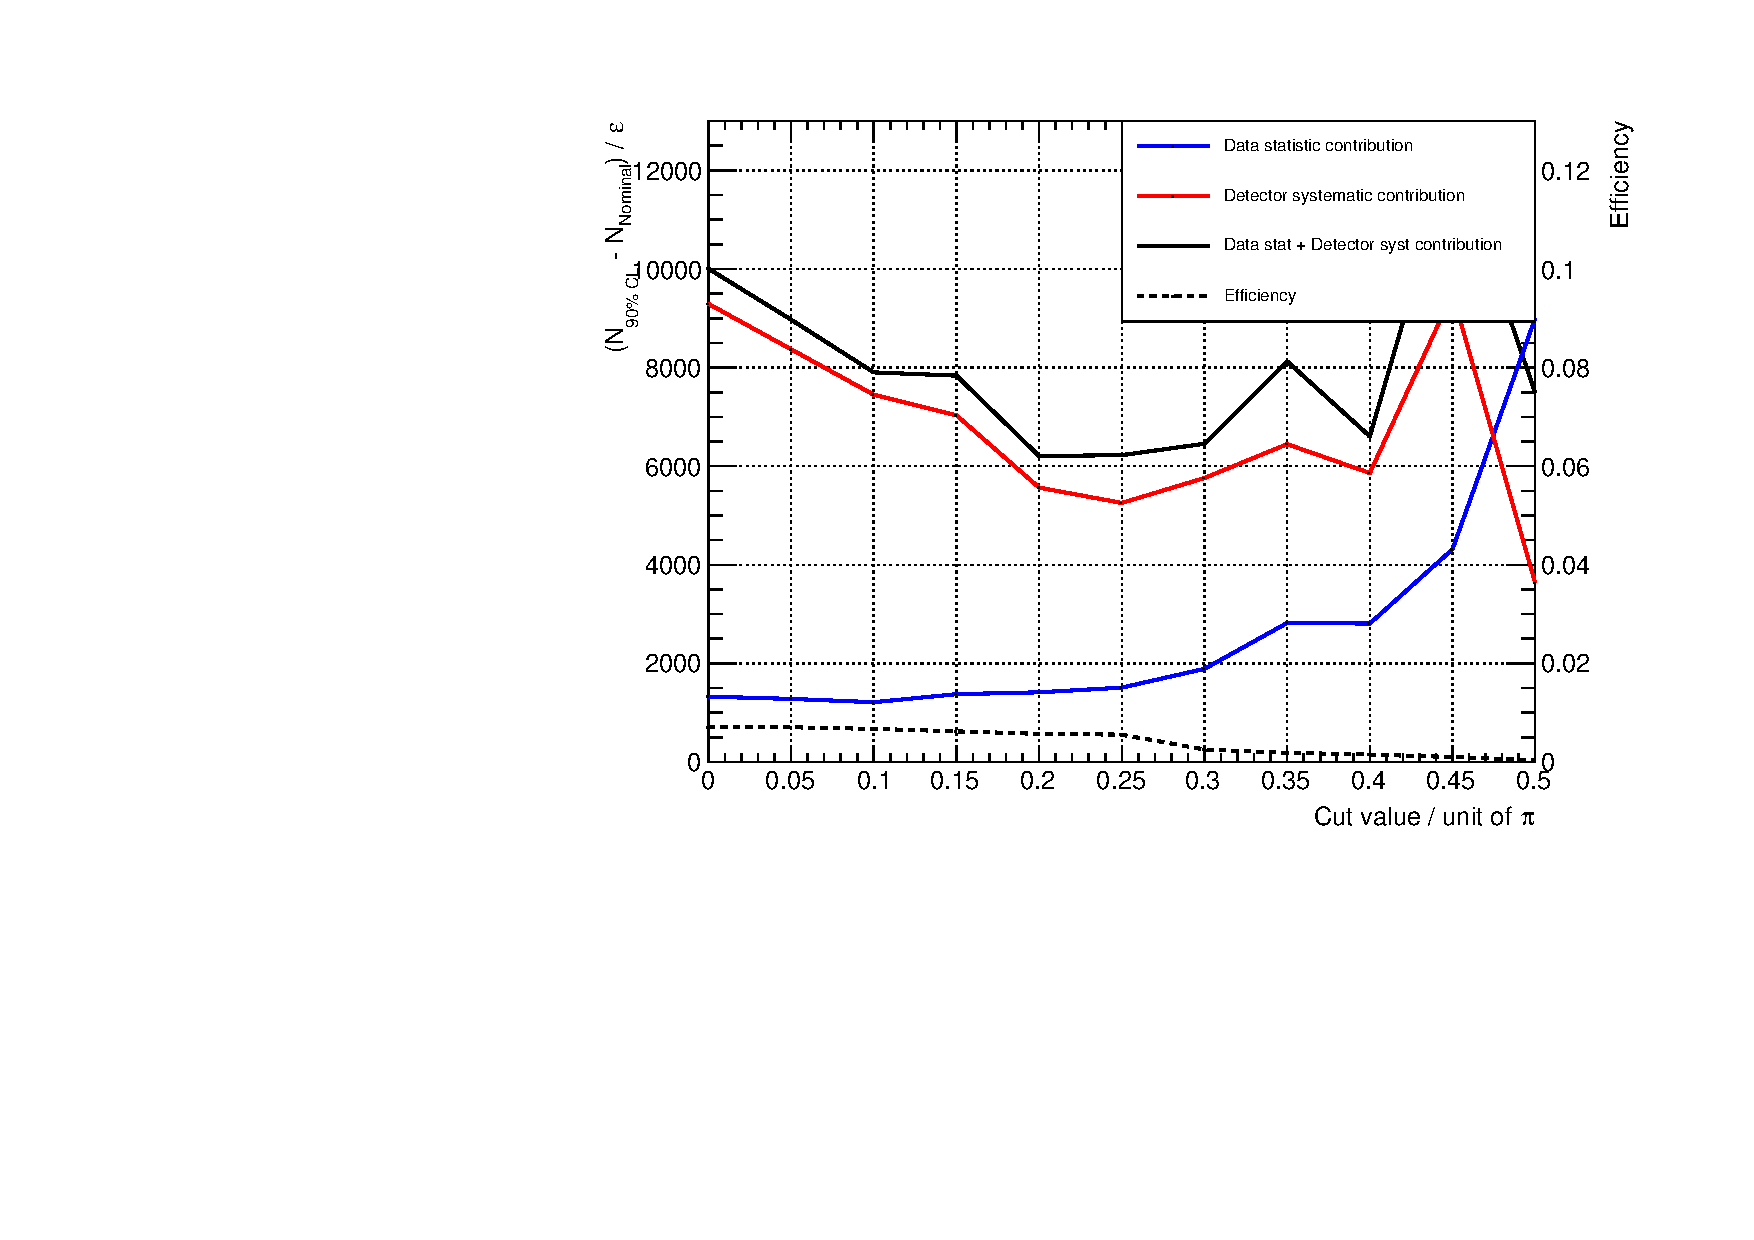
\includegraphics[width=0.8\textwidth]{T2K-TN-254/images/systematics/Optimisation.pdf} 
  \end{adjustbox}
  \caption[Optimisation of the $\varphi$ cut]{Optimisation of the
    $\varphi$ cut, showing the contribution of the data statistic,
    detector systematic errors and efficiency on
    $N_\text{Signal}/\epsilon$, which is proportional to the cross
    section limit.}
  \label{fig:optimisationphi}
\end{figure}

\begin{figure}[ht]
  \begin{adjustbox}{center}
    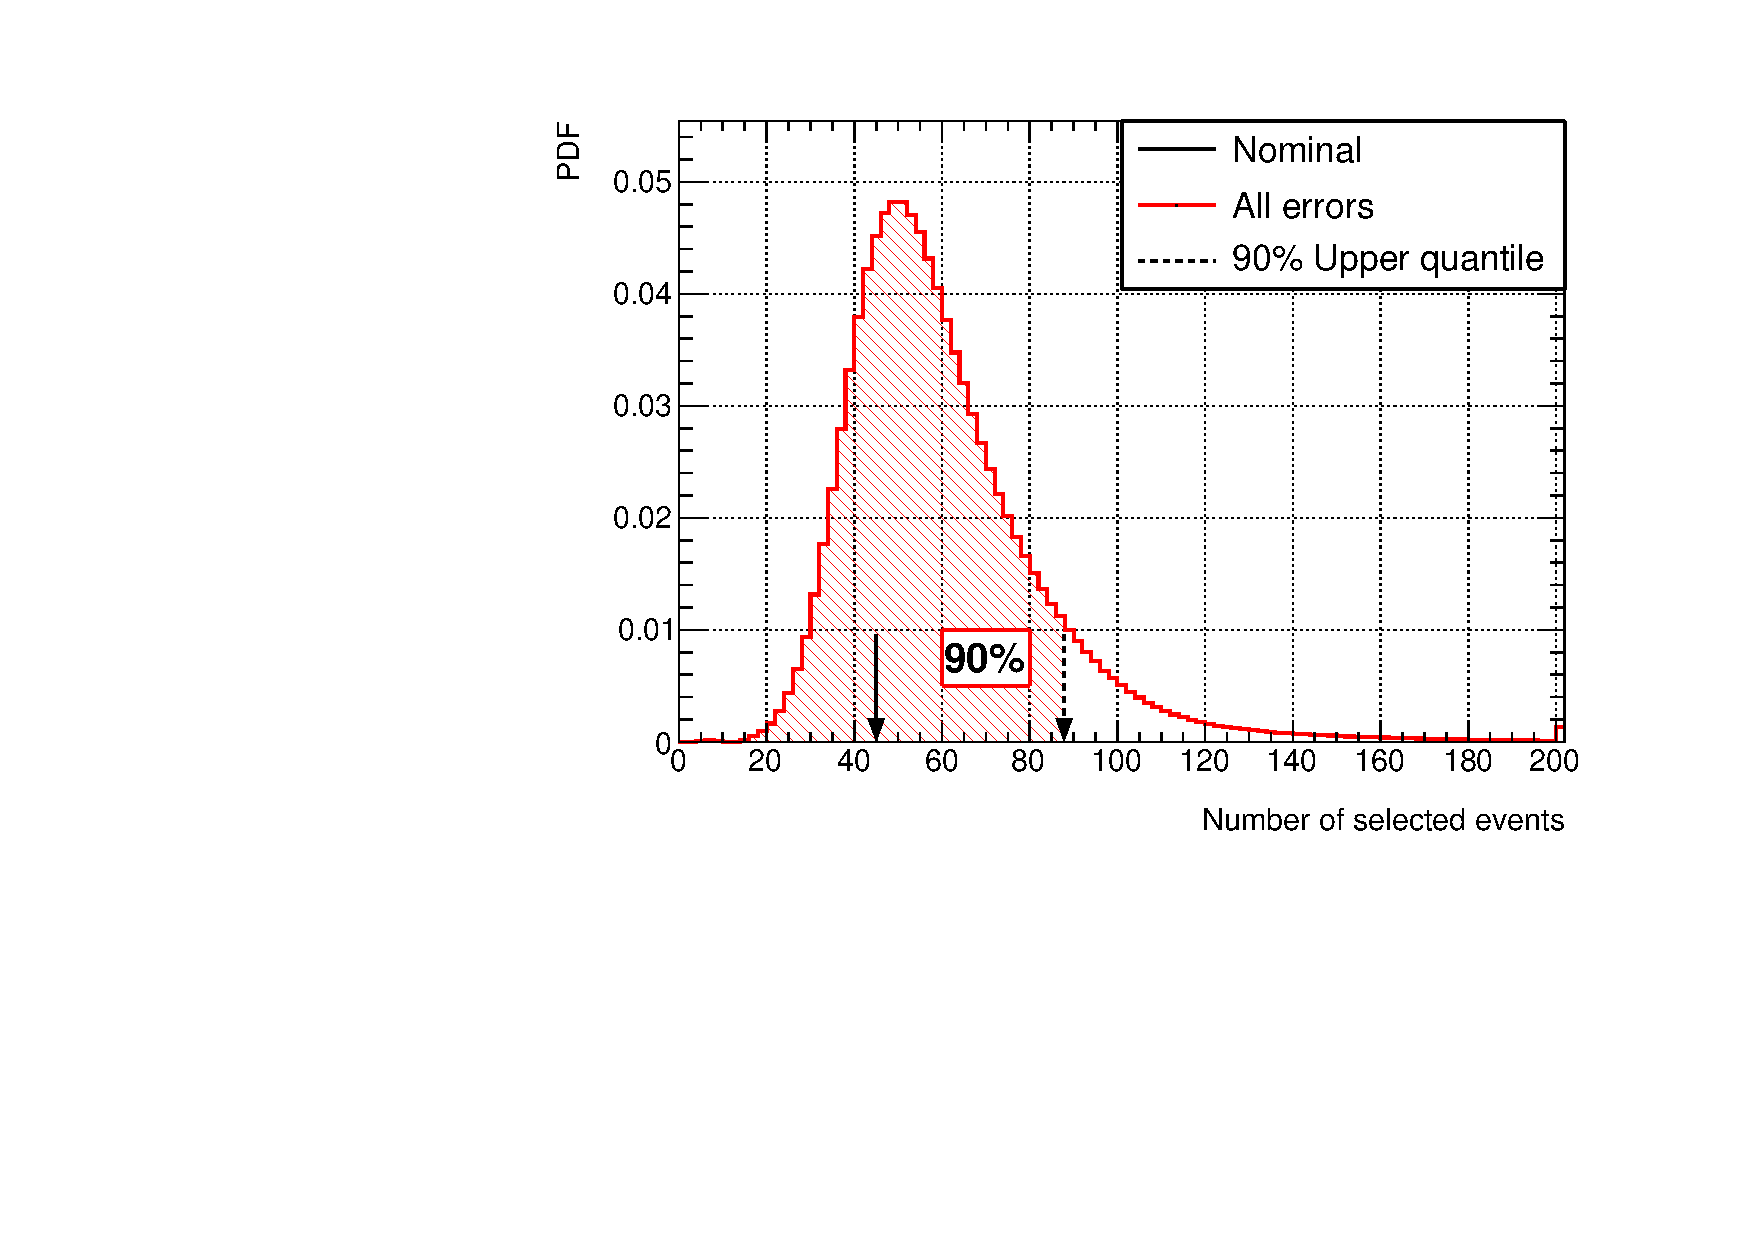
\includegraphics[width=0.8\textwidth]{T2K-TN-254/images/systematics/QuantilePhi.pdf} 
  \end{adjustbox}
  \caption[PDF of the selected number of events from the detector
  uncertainties after the optimised azimuthal cut (with events
  satisfying $-108^{\circ} < \varphi_{\text{photon}} < -72^{\circ}$
  excluded)]{\Gls{PDF} of the selected number of events from the
    detector uncertainties after the optimised azimuthal cut (with
    events satisfying
    $-108^{\circ} < \varphi_{\text{photon}} < -72^{\circ}$ excluded).
    The nominal central value is indicated by the arrow. The $90\%$
    quantile of the \Gls{MC} is also shown.}
  \label{fig:allsystphi}
\end{figure}

\begin{table}[ht]
  \begin{adjustbox}{center}
    \begin{tabular}{lc}
      \toprule
      Systematic error &Relative uncertainty \\ 
      \midrule
      Statistical error on Data (expected) & $\pm 0.14$ \\ 
      Statistical error on Data (observed) & $\pm 0.16$ \\ 
      Statistical error on \Gls{MC}        & $\pm 0.032$ \\ 
      \midrule
      Detector errors                      & $\pm^{0.27}_{0.17}$\\ 
      \midrule
      $C_{A}^{5}$ \Gls{RES} error              &$\pm0.078$ \\ 
      $M_{a}$ \Gls{RES} error                 &$\pm0.089$ \\ 
      Background scale \Gls{RES} error        &$\pm0.023$\\ 
      Nuclear \Gls{RES} ($\Delta$ mass) error &$\pm0.002$\\ 
      \midrule                                
      All errors on single pion production    &$\pm0.20$\\ 
      \midrule
      \Gls{CCQE} errors        & $\pm 0.003 $\\ 
      \Gls{CC}\Gls{nue} error  & $\pm 0.006 $\\ 
      \Gls{DIS} error          & $\pm 0.012 $\\ 
      \Gls{CC} \Gls{COH} error & $\pm 0.001 $\\ 
      \Gls{NC} \Gls{COH} error & $\pm 0.163 $\\ 
      Other \Gls{NC} error     & $\pm 0.032 $\\ 
      \midrule
      All cross section errors (except single pion production) & $\pm 0.036$\\ 
      \midrule
      Flux error & $\pm 0.082$\\ 
      \midrule
      \Gls{FSI} error & $\pm 0.037$\\
      \midrule
      Efficiency error & $\pm 0.0985$ \\
      \midrule
      All errors (except efficiency) & $\pm^{0.33}_{0.23}$ \\ 
      \bottomrule
    \end{tabular}
  \end{adjustbox}
  \caption[Summary of all the errors after the $\varphi$ angle
  cut]{Summary of all the errors after the $\varphi$ angle cut using
    the \Gls{HPD} method.}
  \label{tab:AllErrorPhiCut}
\end{table}


\subsection{Conclusion}
In this section, the importance of each systematic uncertainty and its
effect on the number of selected events were shown. In the case of a
analysis which aims to set a limit, careful characterisation of the
systematic uncertainties is primoridial. This is because the limit is
directly proportional to the total systematic errors (at least in the
case of Gaussian errors). All the asymmetric errors were added
coherently via the described method of discrete convolution. The main,
dominant, error is the detector uncertainty. This error is mitigated
by adding a cut on the reconstructed azimuthal angle of the photon and
removing the photons that comes from under the \Gls{ND}, which have a
large propagation error.

%%% Local Variables:
%%% mode: latex
%%% TeX-master: "Thesis"
%%% End:
